% !TeX root = relazione.tex
\documentclass{article}

\usepackage[utf8]{inputenc}
\usepackage[a4paper, total={15.3 cm, 21.3 cm}]{geometry}
\usepackage{amsmath}
\usepackage{amssymb}
\usepackage{gensymb}
\usepackage{booktabs}
\usepackage{hyperref}
\usepackage{caption}
\usepackage{float}
\usepackage{graphicx}
\usepackage{subfig}
\usepackage{titlesec}
\usepackage{titletoc}
\usepackage{physics}
\usepackage{siunitx}
\usepackage[dvipsnames]{xcolor}

\usepackage{longtable}
\usepackage{tabularx}
\usepackage{calc}
\usepackage{array}
\usepackage{subfiles}
\usepackage{etoolbox}
\usepackage{xparse}


\hypersetup{colorlinks=true,linkcolor=black}
\renewcommand\thesection{\arabic{section}}
\titlecontents{chapter}[1.05em]{\bigskip}
{\contentslabel[\MakeUppercase{\romannumeral\thecontentslabel}]{1em}\enspace\textsc}
{\hspace*{-1em}\textsc}
{\hfill\contentspage}
\titlecontents{section}[1.6em]{\smallskip}
{\thecontentslabel.\enspace}
{}
{\titlerule*[1pc]{.}\contentspage}
\setcounter{tocdepth}{2}




\begin{document}

    \pagenumbering{roman}
    \thispagestyle{empty}

    % First page with uni logo and title
    \begin{center}

        
\includegraphics[width=1.\linewidth]{../../../tools/images/logo.jpg}
        \centering
        \vspace{3cm}

        \uppercase{\Large Relazione di laboratorio:\\ Spettrometro a prisma \par}
        \vspace{3cm}

        \Large Lorenzo Liuzzo, Jiahao Miao, Riccardo Salto\par
        \vspace{1.5cm}

        \Large Novembre 23, 2022

    \end{center}

    \clearpage

    % Table of contents
    \tableofcontents

    \clearpage
    \pagenumbering{arabic}

    % Abstract con una breve descrizione dell'esperimento e i risultati
    \section{Abstract}

        Al fine di determinare l'indice di rifrazione $n$ di un prisma e di verificare la relazione di Cauchy
        \begin{equation}
            n^2 = A \cdot \frac{1}{\lambda^2} + B 
            \label{eq:cauchy1}
        \end{equation}
        \begin{equation}
            n = A \cdot \frac{1}{\lambda^2} + B
            \label{eq:cauchy2}
        \end{equation} 
        (dove i parametri di Cauchy A e B assumono significato fisico distinto tra le due equazioni), 
        è stato utilizzato uno spettrometro per sfruttare gli effetti di riflessione e rifrazione del prisma stesso, 
        note le lunghezze d'onda $\lambda$ dello spettro del mercurio (precedentemente calcolate con uno spettrometro a reticolo),
        per quei particolari valori di $\lambda$. Nella tabella \ref{tabular:spettro}, per ogni riga dello spettro sono riportate il colore, 
        la lunghezza d'onda $\lambda$, l'indice di rifrazione $n$ corrispondente alla lunghezza d'onda con il relativo errore $\sigma_n$.\\
        Sono in oltre state verificate le relazioni lineari con una probabilità associata al $\chi^2$ pari rispettivamente a:
        \[\chi_1 = 30\% \ \ \ \chi_2 = 34\%   \]

        \begin{table}[H]

            \centering
            \begin{tabular}{c c c c}

                \toprule 
                \textbf{colore} & \textbf{$\lambda$[nm]}  & \textbf{n} & \textbf{$\sigma_n$}  \\

                \midrule
                \textcolor{yellow}{Giallo est.}	            &	578,1	&	1,7846 &   0,0008 \\
                \textcolor{Goldenrod}{Giallo int.}     	    &	575,2	&	1,7847 &   0,0014 \\
                \textcolor{green}{Verde}                 	&	545,6	&	1,7915 &   0,0007 \\
                \textcolor{Emerald}{Verde acqua est.}	    &	496,9	&   1,8046 &   0,0007 \\
                \textcolor{cyan}{blu}                    	&	434,8	&   1,8248 &   0,0007 \\
                \textcolor{violet}{Viola est.}             	&	406,8	&   1,8405 &   0,0007 \\
                \textcolor{purple}{Viola int.}	            &	404,0	&   1,8417 &   0,0007 \\
                \bottomrule

            \end{tabular}
            
            \caption{indici di rifrazione per lunghezze d'onda dello spettro del mercurio}
            \label{tabular:spettro}

        \end{table}


    \section{Calibrazione dell'apparato}

        Innanzitutto si è proceduto con la messa a fuoco del cannocchiale rispetto a un obbiettivo sufficientemente lontano 
        affinché fosse valida l'approssimazione di onda piana. A questo punto è stato messo a fuoco il collimatore 
        rispetto alla precedente regolazione del cannocchiale, in modo che fosse verificata l'approssimazione di campo lontano. 
        La piattaforma che regge il prisma è stata poi messa in bolla. A questo punto è iniziata la presa dati.


    \section{Misura dell'angolo $\alpha$ del prisma}

        Per ottenere questa misura è stato sfruttato il fenomeno della riflessione. Tutte le misurazioni delle posizioni angolari sono state effettuate
        su nonio con risoluzione di $1'$ e  successivamente  convertite in radianti. \\
        Tenendo fisso il cannocchiale è stata fatta ruotare la piattaforma affichè l'immagine della fenditura riflessa fosse centrata 
        con il crocifilo. Una volta misurata sul nonio la posizione angolare $\theta_1$, la piattaforma è stata ruotata affichè il crocifilo 
        centrasse l'immagine reale, ed è stata annotata la posizione angolare $\theta_2$.
        
        È stata utilizzata la risoluzione dello strumento come incertezza associata alla singola misura $\sigma = 0.02$ ° (pari a $3 \cdot 10^{-4}$ rad). 
        A questo punto è stata calcolata la differenza $\Delta\theta$ tra i due angoli, alla quale è stata associata come incertezza $\sigma_{\Delta\theta}$ 
        la somma in quadratura delle singole incertezze sulle misure angolari, pari a: \[ \sigma_{\Delta\theta} = 0.02 ^\circ \]
        È stato possibile ricavare l'angolo $\alpha$ dalla relazione geometrica: \[ \alpha = 180 ^\circ - \Delta\theta \]

        La misura è stata ripetuta 8 volte e in tabella \ref{tabular:delta theta} sono riportate le misure degli angoli misurati $\theta_1$ e $\theta_2$ 
        e la loro differenza $\Delta\theta$. A questo punto è stata fatta una media dei $\Delta\theta$ ottenendo come valore:
        \[ \Delta\theta = 240,03^\circ \] a cui è stata associata come incertezza la deviazione standard della media del set di misure:
        \[ \sigma_{\Delta\theta} = 0,03^\circ \]
        A questo punto è stato possibile valutare l'angolo $\alpha$, ottenendo un valore pari a: 
        \[\alpha = (60,03\pm 0,03)^\circ = (1,0477\pm 0,0006)\, \mathrm{rad}\]

        \begin{table}[H]

            \centering
            \begin{tabular}{c c c}

                \toprule 
                $\theta_1 [^\circ]$ & $\theta_2 [^\circ]$  & $\Delta\theta [^\circ]$  \\
                
                \midrule
                66,58	&	306,73	&	240,15\\
                66,40	&	306,52	&	240,12\\
                39,82	&	279,78	&	239,97\\
                37,20	&	277,20	&	240,00\\
                34,83	&	274,75	&	239,92\\				
                35,60	&	275,73	&	240,13\\				
                35,70	&	275,65	&	239,95\\
                47,80	&	287,78	&	239,98\\
                \bottomrule

            \end{tabular}

            \caption{valori degli angoli misurati $\theta_1$ e $\theta_2$ e della loro differenza $\Delta\theta$}
            \label{tabular:delta theta}

        \end{table}


    \section{Misura dell'indice di rifrazione del prisma}

        Per prima cosa è stato misurato l'angolo di zero $\theta_0$. La misura è stata ripetuta 10 volte e con una media è stato ottenuto come valore:
        \[ \theta_0 = (178,67\pm 0,02) ^\circ = (3,118 \pm 0,0003)\, \mathrm{rad} \]
        Dove come errore associato è stata utilizzata la risoluzione al posto della  deviazione standard della media delle 10 misure 
        perché la deviazione standard risulta inferiore alla risoluzione dello strumento di misura. 
        Le misure di $\theta_0$ sono riportate in tabella \ref{tabular:theta zero}.
            
        \begin{table}[H]

            \centering
            \begin{tabular}{c}

                \toprule 
                $\theta_0$° \\

                \midrule
                178,667\\
                178,683\\
                178,700\\
                178,650\\
                178,633\\
                178,667\\
                178,683\\
                178,667\\
                178,700\\
                178,650\\
                \bottomrule

            \end{tabular}

            \caption{misure dell'angolo di zero $\theta_0$}
            \label{tabular:theta zero}

        \end{table}

        A questo punto è stato misurato per ogni colore l'angolo di deviazione minima. 
        Osservando una particolare riga dello spettro, è stata fatta ruotare la piattaforma contenete il prisma seguendo la riga col cannocchiale 
        fino a che questa non invertiva il senso dello spostamento. È stata quindi segnata la posizione angolare $\theta(\lambda)$ corrispondente 
        al punto in cui avveniva l'inversione. La misura è stata ripetuta 5 volte per ogni lunghezza d'onda. 
        In tabella \ref{tabular:theta misure} sono riportate per ogni colore dello spettro i valori raccolti in questa fase espressi in gradi.

        \begin{table}[H]

            \centering
            \begin{tabular}{c c c c c c c}

                \toprule 
                giallo est. [°] & gialli int. [°]& verde acqua [°]& verde [°]& blu [°]& viola est. [°]& viola int. [°]  \\
                
                \midrule
                112,13	&	112,05	&	111,42	&	109,70	&	106,93	&	104,67	&	104,48\\
                112,37	&	112,63	&	111,47	&	109,58	&	106,82	&	104,63	&	104,52\\
                112,40	&	112,62	&	111,33	&	109,62	&	106,97	&	104,77	&	104,60\\
                112,25	&	112,00	&	111,37	&	109,80	&	107,02	&	104,65	&	104,42\\
                112,20	&	112,02	&	111,40	&	109,70	&	106,83	&	104,62	&	104,43\\
                \bottomrule

            \end{tabular}

            \caption{misure relative degli angoli di deviazione minima $\theta(\lambda)$ per ogni colore dello spettro del mercurio}
            \label{tabular:theta misure}

        \end{table}

        Dai dati raccolti, per ogni lunghezza d'onda, è stato ottenuto un valore medio $\theta(\lambda)_m$ la cui incertezza $\sigma_{\theta(\lambda)_m}$ 
        è stata stimata attraverso la deviazione standard della media delle misure. L'angolo di deviazione minima $\delta$ è stato trovato sottraendo 
        alla posizione relativa la posizione di zero $\theta_0$. L'incertezza su $\delta_m(\lambda)$, $\sigma_{\delta_m(\lambda)}$, è stata ottenuta sommando 
        in quadratura i singoli errori dei due addendi. A questo punto, tramite la relazione:
        \[n(\lambda) = \frac{sin(\frac{\delta_m(\lambda) + \alpha}{2})}{sin(\frac{\alpha}{2})}\]
        è stato ricavato l'indice di rifrazione del prisma per ogni lunghezza d'onda. 
        Con errore associato $\sigma_n$ ottenuto dalla somma in quadratura dei due errori $\sigma_1$ e $\sigma_2$:
        \[\sigma_1 = \sigma_{\delta} \cdot \frac{\cos(\frac{\alpha + \delta}{2})}{2\sin(\frac{\alpha}{2})} \]
        \[\sigma_2 = \sigma_{\alpha}\cdot \frac{\cos(\frac{\alpha + \delta}{2})\sin(\frac{\alpha}{2}) - 
                    \sin(\frac{\alpha + \delta}{2})\cos(\frac{\alpha}{2})}{2\sin^2(\frac{\alpha}{2})} \]
        In tabella \ref{tabular:misure delta e n} sono riportate per ogni colore le misure dell'angolo di deviazione minima e dell'indice di rifrazione, con le loro incertezze.    


        \begin{table}[H]

            \centering
            \begin{tabular}{ c c c c c  }

                \toprule 
                colore & $\delta$ rad & $\sigma_{\delta}$rad & $n$ & $\sigma_n$   \\
                
                \midrule
                \textcolor{yellow}{Giallo est.}	        &   1,159	&	0,001	&	1,7846 &   0,0008\\
                \textcolor{Goldenrod}{Giallo int.}      &   1,159	&	0,003	&	1,7847 &   0,0014\\
                \textcolor{green}{Verde}                &   1,1741	&	0,0005	&	1,7915 &   0,0007\\
                \textcolor{Emerald}{Verde acqua est.}	&   1,2041	&	0,0007	&	1,8046 &	  0,0007\\
                \textcolor{cyan}{blu}                   &   1,2524	&	0,0008	&	 1,8248 &	  0,0007\\
                \textcolor{violet}{Viola est.}          &   1,2916	&	0,0005	&	1,8405 &	  0,0007\\
                \textcolor{purple}{Viola int.}	        &   1,2947	&	0,0007	&	 1,8417 &	  0,0007\\
                \bottomrule

            \end{tabular}

            \caption{valori dell'angolo di deviazione minima e dell'indice di rifrazione per ogni colore dello spettro del mercurio}
            \label{tabular:misure delta e n}

        \end{table}

        A questo punto è stato possibile verificare la validità delle relazioni di Cauchy \ref{eq:cauchy1} e \ref{eq:cauchy2}.
        Sono quindi state fatte due regressioni lineari con i valori delle lunghezze d'onda tabulate in modo da ottenere i coefficienti angolari $a_1$ e $a_2$
        delle rette per poter trasferire l'incertezza delle lunghezze d'onda misurate con lo spettrometro a reticolo sull'asse y. 
        In questo modo sono state effettuate di nuovo le due regressioni lineari pesate, utilizzando come lunghezze d'onda quelle precedentemente misurate. 
        Sono stati trovati i seguenti coefficienti:
        \[a_1 = (6,56 \pm 0,08 )10^{-14}\ m^2\ \ \ \ b_1 = (2,990\pm 0,004)\]
        \[a_2 = (1,81 \pm 0,02 )10^{-14}\ m^2\ \ \ \ b_2 = (1,731\pm 0,001)\]

        Per entrambe le regressioni è stato effettuato un test di $\chi^2$ che ha dato come livello di confidenza per le relazioni 
        \ref{fig:Cauchy_1} e \ref{fig:Caychy_2} rispettivamente il $30\%$ e il $34\%$. 
        In Figura IWIBVIURBV sono riportati i grafici delle due regressioni. 

        \begin{figure}

            \centering
            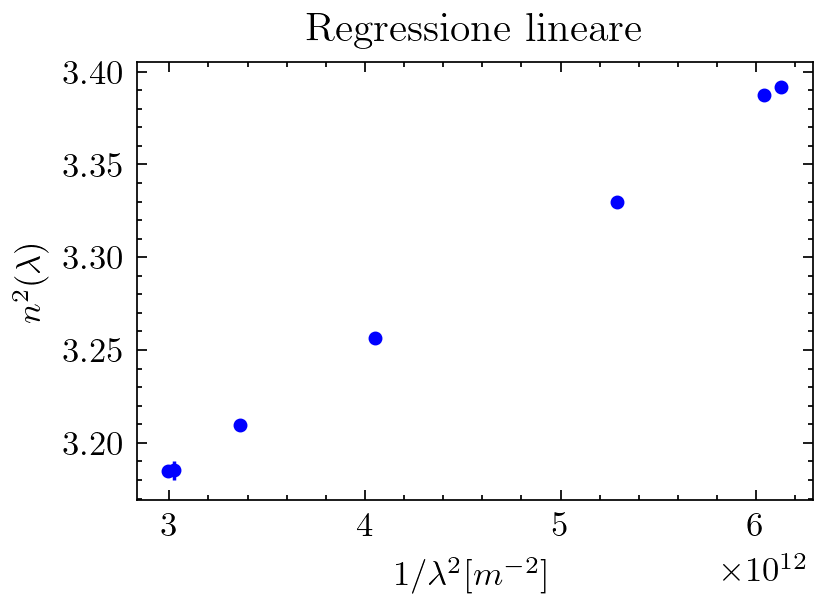
\includegraphics{../images/Cauchy_1.png}
            \caption{Relazione di Cauchy $n^2$}
            \label{fig:Cauchy_1}

        \end{figure}

        \begin{figure}

            \centering
            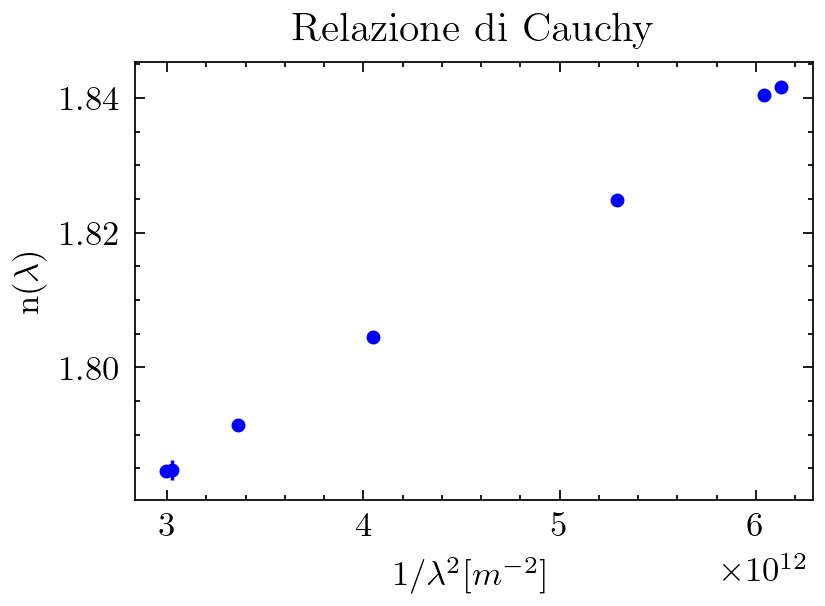
\includegraphics{../images/Cauchy_2.png}
            \caption{Relazione di Cauchy n}
            \label{fig:Cauchy_2}

        \end{figure}


\end{document}